\scanpage{619}
\mspage{613}

Let us return to diagram (130), I say that the homomorphism
\diagram{\begin{tikzcd}
 \gamma_{\rho,\sigma}\arrow[r]\arrow[d,phantom,"\Vert"] & N^*_{\rho}/\{\pm1\}\\
 \Gamma_{\mathbb Q}^{\sim}
\end{tikzcd}}
\uline{does not lift} to a homomorphism from $\gamma_{\rho,\sigma}$ to
$\underset{\inserted{\widetilde\gamma_{\rho,\sigma}}}{N^*_{\rho}}$
--- in other words, that the extension of $\gamma_{\rho,\sigma}$ by
$\{\pm1\}=\mu$ which it defines is not trivial. To identify this
extension, let us consider the diagram
\margin{\uline{N.B.}}
\[
(144)\qquad
\diagram{\begin{tikzcd}[column sep=large,row sep=huge]
 \mathcal M^![0]=Z^!_{\rho,\sigma}\arrow[rr,"\text{canonical}"]
 &&\gamma_{\rho,\sigma}=Z^!_{\rho,\sigma}/L_0^{\Pi}
       \arrow[r,"\text{homomorphism }(130)"]
 &N^*_{\rho}/\{\pm1\}\\
 S_0\Gamma^!_{\rho,\sigma}
       \arrow[u,"{\text{canonical}\quad(u,a,b)\mapsto u}"']
 &\inserted{\unsure{S_0}\Gamma_{\rho,\sigma}\quad\text{(without !)}}
       \arrow[ur,very thick,"{\substack{\text{canonical}\\\unsure{\text{(passage to the quotient)}}}}"']
 &&\\
 S_0^{\Pi}\Gamma^!_{\rho,\sigma}\arrow[u,hook,"\text{inclusion}"']
       \arrow[ur,hook,dashed,"\text{inclusion}"']\arrow[rrr]
 &&&N^*_{\rho}\arrow[uu]
\end{tikzcd}}
\]
which shows that we have a diagram of cartesian squares
\[
(145)\quad\deleted{\unsure{(146)|(144)}}\qquad
\diagram{\begin{tikzcd}[column sep=large,row sep=huge]
 \mathcal M(0)\arrow[r,hook]\arrow[dr,phantom,"\mathrm I" description]
 &\mathcal M^![0]=Z^!_{\rho,\sigma}\arrow[r,"\text{epimorphism}"]
       \arrow[dr,phantom,"\mathrm {II}" description]
 &\gamma_{\rho,\sigma}\arrow[r,hook]
       \arrow[dr,phantom,"\mathrm {III}" description]
 &N^*_{\rho}/\{\pm1\}\\
 \mathcal M(0)^{\sim}\arrow[u]\arrow[r,hook]
 &S_0^{\Pi}\Gamma^!_{\rho,\sigma}\arrow[u,"2"]\arrow[r]
 &\widetilde\gamma_{\rho,\sigma}\arrow[u,"2"]\arrow[r,hook]
 &N_{\rho}^{\unsure{*|d}}\arrow[u,"2"]
\end{tikzcd}}
\]
where $\mathcal M(0)^{\sim}$ is \unsure{defined|defined} as the extension of
$\mathcal M(0)$ by $\mu$ induced by the extension
$S_0^{\Pi}\Gamma^!_{\rho,\sigma}$ of $\mathcal M^![0]$,
which is thus identified \unsure{also} with the \unsure{inverse|inverse} image of

\scanpage{620}

the extension $\widetilde\gamma_{\rho,\sigma}$ of $\gamma_{\rho,\sigma}$ by $\mu$,
under the composite isomorphism
\diagram{\begin{tikzcd}
 \mathcal M(0)\arrow[r,"\sim"] & \gamma_{\rho,\sigma}.
\end{tikzcd}}
So the extension $\widetilde\gamma_{\rho,\sigma}$ of $\gamma_{\rho,\sigma}$ by
$\mu$ is identified \unsure{naturally|naturally} with the extension $\mathcal M(0)^{\sim}$ of
$\mathcal M(0)$ by $\mu$ which we have more or less convinced ourselves
was not trivial.

Here is another way of obtaining the canonical homomorphism
\diagram{\begin{tikzcd}
 \gamma_{\rho,\sigma}\arrow[r] & N^*_{\rho}/\pm1,
\end{tikzcd}}
and the extension $\widetilde\gamma_{\rho,\sigma}$ of $\gamma_{\rho,\sigma}$.
Let us consider
\[
 (146)\qquad N_{\rho}^{*!}=N^*_{\rho}\cap\mathcal M^!
\]
We then have
\[
 (147)\qquad
 N_{\rho}^{*!}\cap\mathcal G^+
 =\operatorname{Ker}\bigl(N_{\rho}^{*!}\longrightarrow
     \underbrace{\gamma_{\rho,\sigma}}_{\Gamma_{\mathbb Q}^{\unsure{\sim}}}\bigr)
 =L_{\rho}\cap\Pi=\mu
\]
on the other hand the homomorphism
\[
 (148)\qquad
 \diagram{\begin{tikzcd}
 N_{\rho}^{*!}\arrow[r] & \gamma_{\rho,\sigma}
 \end{tikzcd}}
 \quad\text{is an \uline{epimorphism}}
\]
For \deleted{for $\forall$} it suffices to see that \inserted{for}
$\forall\,u\in\mathcal M(0)$, there exists an element of $N_{\rho}^{*!}$
which is congruent to it, \inserted{modulo $\mathcal G$} Now we have
\[
 u(\rho)=\operatorname{int}(\alpha)(\rho)
 \deleted{=\unsure{\operatorname{int}(\alpha_0\varepsilon_3[\tau])(\rho)}}
\]
\inserted{with $\alpha\in\deleted{\unsure{\widehat\Pi_{\tau}}}
 \widehat\Pi_{\tau}=\{1,\tau\}.\widehat\Pi$,}
if $\varepsilon_3(u)=1$ i.e. $\alpha\in\widehat\Pi$,
$\alpha^{-1}u\in\deleted{\unsure{Z}}Z_{\rho}\subset N^*_{\rho}$
does the job. If \deleted{$\unsure{\varepsilon_3(u)=-1}$}
\inserted{$\varepsilon_3\unsure{=|\ne}-1$}, we have
\deleted{we have}
\[
 \deleted{\alpha=\alpha_0}\quad\alpha=\alpha_0\tau,\qquad\alpha_0\in\widehat\Pi.
\]
and we have
\[
 u(\rho)=\alpha(\rho)=
 \alpha_0\bigl(\underbrace{\tau(\rho)}_{\sigma(\rho^{-1})}\bigr)
 =\alpha_0(\sigma(\rho^{-1}))\quad\deleted{so}
\]
so
\[
 (\sigma^{-1}\alpha_0^{-1}u)(\rho)=\rho^{-1}
 \quad\text{so}\quad\sigma^{-1}\alpha_0^{-1}u\in N^*_{\rho}.
\]
\unsure{OK.}

\scanpage{621}
\mspage{614}

So we have an \unsure{exact} sequence

\( (149) \)\quad
\diagram{\begin{tikzcd}[column sep=small,row sep=small]
1 \arrow[r] & \mu \arrow[r] & Z_\rho^{*!} \arrow[r] & \gamma_{\rho,\sigma} \arrow[r] \arrow[d,phantom,"\rotatebox{90}{$\simeq$}"] & 1 \\
& & (\simeq\widetilde{\gamma}_{\rho,\sigma}) & \widetilde{\Gamma}_{\mathbb Q} &
\end{tikzcd}}

which makes $Z_\rho^{*!}$ a $\mu$-extension of $\gamma_{\rho,\sigma}$,
hence a canonical homomorphism

\diagram{\begin{tikzcd}
\gamma_{\rho,\sigma}\simeq Z_\rho^{*!}/\mu \arrow[r] & N_\rho^*/\mu
\end{tikzcd}}

which, of course, is none other than the first homomorphism (130).

$9^\circ)$ \uline{Recapitulation on the universal case}.

Finally, I have the impression that I have again made long detours and
\unsure{contortions}, to finally get lost in the sands, and lose
the thread a little. So I am going to recapitulate what seems essential to me.

\textcircled{a}
\[
(1)\qquad Z_{\rho,\sigma}\simeq\mathcal M(0).L_0^{\mathcal G}
\inserted{=\mathcal M[0]}\ \deleted{\illegible{1}}\ \inserted{
\text{(operating on }\widehat{\mathcal G}^{+}\text{ by operation induced by }\unsure{\text{the adjoint}}\text{)}}
\]

we distinguish inside it a sub\unsure{group} of index $2$
\[
(2)\qquad Z_{\rho,\sigma}^{!}\simeq\mathcal M(0).L_0^{\Pi}.
\]

\scanpage{622}

We have
\[
(3)\qquad \unsure{G}_{\rho,\sigma}\simeq\mathcal M
\]

and, \deleted{the homomorphisms} more precisely, the diagram

\( (4) \)\quad
\diagram{\begin{tikzcd}[column sep=small,row sep=large]
1 \arrow[r] & L_0 \arrow[r] \arrow[d,hook] & Z_{\rho,\sigma} \arrow[r] \arrow[d,hook] & \gamma_{\rho,\sigma} \arrow[r] \arrow[d,equal] & 1 \\
1 \arrow[r] & \mathcal G_{\rho,\sigma}^{+\wedge} \arrow[r] & G_{\rho,\sigma} \arrow[r] & \gamma_{\rho,\sigma} \arrow[r] & 1
\end{tikzcd}}

is identified with the diagram

\( (4\text{ bis}) \)\quad
\diagram{\begin{tikzcd}[column sep=small,row sep=large]
1 \arrow[r] & L_0^{\mathcal G} \arrow[r] \arrow[d,hook] & \overbrace{\mathcal M[0]}^{\inserted{\mathcal M(0).L_0^{\mathcal G}}} \arrow[r] \arrow[d,hook] & \widetilde{\Gamma}_{\mathbb Q} \arrow[r] \arrow[d,phantom,"\rotatebox{90}{$\simeq$}"] & 1 \\
1 \arrow[r] & \widehat{\mathcal G}^{+} \arrow[r] & \mathcal M \arrow[r] & \widetilde{\Gamma}_{\mathbb Q} \arrow[r] & 1.
\end{tikzcd}}

Moreover, the homomorphisms

\( (5) \)\quad
\diagram{\begin{tikzcd}[column sep=large,row sep=small]
& \mu \\
\gamma_{\rho,\sigma} \arrow[ru,"{\varepsilon_\gamma'=\varepsilon_\gamma^\rho}"] \arrow[r] \arrow[rd,"{\varepsilon_\gamma''=\varepsilon_\gamma^{\unsure{\rho|\sigma}}}"'] & \widehat{\mathbb Z}^{*} \\
& \mu
\end{tikzcd}}

are identified:

\( (5\text{ bis}) \)\quad
\diagram{\begin{tikzcd}[column sep=large,row sep=small]
& & \mu \\
\widetilde{\Gamma}_{\mathbb Q} \arrow[r,Rightarrow,"\chi"] \arrow[urr,bend left=15,"\varepsilon_3"] \arrow[drr,bend right=15,"\varepsilon_2"'] & \widehat{\mathbb Z}^{*} \arrow[ur] \arrow[dr] & \\
& & \mu.
\end{tikzcd}}

\textcircled{b}\quad We have

\margin{$/$}
\[
(6)\qquad N_\sigma^*=
\left\{u\in\unsure{\mathcal M}\ \middle|\ u(\sigma)=\deleted{\unsure{\varepsilon_2(u)}}\sigma^{\varepsilon_2(u)}
\begin{aligned}
&\bigl(=\varepsilon_2(u).\sigma\bigr)\\
&\inserted{=\varepsilon_2[\tau](\sigma)}\\
&\inserted{=\varepsilon_2[\tau'](\sigma)}
\end{aligned}
\right\}
\]

\deleted{\unsure{Let us put}} and
\[
(7)\qquad
\left\{\begin{aligned}
N_\sigma^*\cap\widehat{\mathcal G}
  &=\mathbb D_\sigma=\{1,\tau\}.L_\sigma=\{1,\tau'\}.L_\sigma\\
N_\sigma^*\cap\mathcal G^{+\wedge}
  &= L_\sigma\qquad(\simeq\mathbb Z/4\mathbb Z)\\
N_\sigma^*\cap\Pi&=\mu\\
N_\sigma^*\cap\Pi_0&=\{1\}
\end{aligned}\right.
\qquad .
\]

\scanpage{623}
\mspage{615}

Let us put
\[
(8)\qquad
\left\{\begin{aligned}
\mathcal M_0^!&=\mathcal M(0).\Pi_0
\subset\mathcal M^!=\mathcal M(0).\Pi
=\operatorname{Ker}(\mathcal M\to\mathcal G_3)\\
\text{so that}\qquad
\mathcal M^!&\simeq\mathcal M_0^!\times\mu
\end{aligned}\right.
\]

and
\[
(9)\qquad
\left\{\begin{aligned}
\mathcal M(1/2)
&\overset{\mathrm{dfn}}=
\deleted{\unsure{A}}N_{\sigma\deleted{\unsure{\rho}}0}^{*!}
\overset{\mathrm{dfn}}=
\deleted{\unsure{Z_\sigma\mathcal M_0}}N_\sigma^*\cap\mathcal M_0^!\\
N_\sigma^{*!}&=N_\sigma^*\cap\mathcal M^!
=\deleted{\unsure{\mathcal M(1/2)|\mathcal M(0)}\times\mu},
\end{aligned}\right.
\]

then the homomorphism \deleted{\unsure{from}} $\mathcal M\to\gamma_{\rho,\sigma}$
induces an \uline{isomorphism}

\( (10) \)\quad
\diagram{\begin{tikzcd}
\mathcal M(1/2)=N_{\sigma0}^{*!} \arrow[r,"\sim"] & \gamma_{\rho,\sigma}
\end{tikzcd}}

so we have splittings into $1/2$ \unsure{direct} products
\[
(11)\qquad
\left\{\begin{aligned}
.\ \mathcal M^{\deleted{\unsure{!}}}
  &\simeq\mathcal M(1/2).\mathcal G^{+\wedge}\\
\mathcal M^!&\simeq\mathcal M(1/2).\Pi\\
\mathcal M_0^!&\simeq\mathcal M(1/2).\Pi_0\\
N_\sigma^{*!}&\simeq\mathcal M(1/2)\times\mu\\
N_\sigma^*&\simeq\mathcal M(1/2).L_\sigma
\end{aligned}\right.\quad,\quad\text{and}
\]

\( (12) \)\quad
\diagram{\begin{tikzcd}
\gamma_{\rho,\sigma} \arrow[r,"\sim"] & \mathcal M(1/2)=N_{\sigma0}^{*!} \arrow[r,hook] & N_\sigma^*.
\end{tikzcd}}

\figure{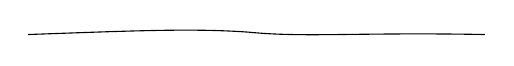
\begin{tikzpicture}
\draw (0,0) .. controls (1.4,.05) and (2.1,.08) .. (2.8,.03)
.. controls (3.5,-.04) and (4.2,.03) .. (5.8,0);
\end{tikzpicture}}

\textcircled{c}\quad We have
\[
(13)\qquad
N_\rho^*=\left\{u\in\mathcal M\mid u(\rho)=\rho^{\varepsilon_3(u)}\right\}
\quad\inserted{\bigl(=\varepsilon_3[\tau'](\rho)\bigr)}
\]

and
\[
(14)\qquad
\left\{\begin{aligned}
N_\rho^*\cap\widehat{\mathcal G}
  &=\mathbb D_\rho=\{1,\tau'\}.L_\rho\\
N_\rho^*\cap\mathcal G
  &=L_\rho\qquad(\simeq\mathbb Z/6\mathbb Z)\\
N_\rho^*\cap\Pi&=\mu\\
N_\rho^*\cap\Pi_0&=\{1\}
\end{aligned}\right.\qquad .
\]

\scanpage{624}

Let
\[
(15)\qquad
N_{\rho0}^{*!}\overset{\mathrm{dfn}}=N_\rho^*\cap\mathcal M_0^!,
\qquad N_\rho^{*!}=N_\rho^*\cap\mathcal M^!.
\]

we find
\[
(16)\qquad
N_{\rho0}^{*!}\subset Z_\rho
=\operatorname{Cent}_{\unsure{\mathcal M(0)|\mathcal M}}(\rho)
=\operatorname{Cent}_{\mathcal M}(L_\rho)
\]

and we also note
\[
(17)\qquad N_{\rho,0}^{*!}=Z_{\rho0}^{!}=\mathcal M'(-\bar j).
\]

We see that the homomorphism $\mathcal M\to\gamma_{\rho,\sigma}
=\widetilde{\Gamma}_{\mathbb Q}$ induces an \uline{isomorphism}

\( (\unsure{18}) \)\quad
\diagram{\begin{tikzcd}[column sep=large,row sep=small]
\mathcal M'(-\bar j)=Z_{\rho,0}^{!} \arrow[r,"\sim"] &
\gamma'_{\rho,\sigma}=\widetilde{\Gamma}_{\mathbb Q}
\arrow[d,phantom,"{\rotatebox{90}{$=$}\ \mathrm{dfn}}"]\\
&\{\gamma\in\gamma_{\rho,\sigma}\mid\varepsilon_3(\gamma)=1\}
\end{tikzcd}}

from which we deduce splittings into semidirect products
(or even direct products)
\[
(19)\qquad
\left\{\begin{aligned}
\mathcal M'&\simeq\mathcal M'(-\bar j).\mathcal G^{+\wedge}\\
\mathcal M^{\prime!}&\simeq\mathcal M'(-\bar j).\Pi\\
\mathcal M_0^{\prime!}&\simeq\mathcal M'(-\bar j).\Pi_0\\
Z_\rho^!\unsure{=|\simeq}\unsure{N_\rho^{*!}}
  &\simeq\mathcal M'(-j)\times\mu\\
\deleted{\unsure{N_\rho^*}}Z_\rho
  &\simeq\mathcal M'(-j)\times L_\rho
\end{aligned}\right.\qquad .
\]

\deleted{The correspondence between}
\diagram{\begin{tikzcd}
\deleted{\unsure{\mathcal M^{!\prime}[0]|\mathcal M^{\prime!}[0]}}
\arrow[r,"{\deleted{\sim}}"] & \deleted{\gamma'_{\rho,\sigma}}
\end{tikzcd}}
\deleted{and}
\diagram{\begin{tikzcd}[column sep=small]
\deleted{\mathcal M(-j)} \arrow[r,phantom,"{\deleted{\subset}}"]
\arrow[rr,bend right=25,"{\deleted{\sim}}"'] &
\deleted{N_\rho^*} & \deleted{\gamma_{\rho,\sigma}}
\end{tikzcd}}
\deleted{is defined by the map}

\deleted{\( (18) \)}\quad
\diagram{\begin{tikzcd}
\deleted{\unsure{\mathcal M^{!\prime}[0]|\mathcal M^{\prime!}[0]}}
\arrow[r] & {}
\end{tikzcd}}